% Template adapted from https://github.com/jgm/pandoc-templates/blob/master/default.latex
% To be used with XeLaTex in memoiR
%%%%%%%%%%%%%%%%%%%%%%%%%%%%%%%%%%%%%%%%%%%%%%%%%%%%%%%%%%%%%%%%%%%%%%%%%%%%%%%%%%%%%%%%%

% Options for packages loaded elsewhere
\PassOptionsToPackage{unicode=true}{hyperref}
\PassOptionsToPackage{hyphens}{url}
\PassOptionsToPackage{dvipsnames,svgnames*,x11names*}{xcolor}
% Right to left support


\documentclass[
  12pt,
  american,
  a4paper,
  extrafontsizes,onecolumn,openright
  ]{memoir}

% Double (or whatever) spacing

% Math
\usepackage{amssymb, amsmath}
% mathspec: arbitrary math fonts
\usepackage{unicode-math}
\defaultfontfeatures{Scale=MatchLowercase}
\defaultfontfeatures[\rmfamily]{Ligatures=TeX,Scale=1}

% Fonts
\usepackage{lmodern}
\usepackage{fontspec}
% Main font
% Specific sanserif font
% Specific monotype font
% Specific math font
% Chinese, Japanese, Corean fonts

% Use upquote for straight quotes in verbatim environments
\usepackage{upquote}
% Use microtype
\usepackage[]{microtype}
\UseMicrotypeSet[protrusion]{basicmath} % disable protrusion for tt fonts

% Verbatim in note

% Color links
\usepackage{xcolor}

% Strikeout

% Necessary for code chunks

% Listings package

% Tables
\usepackage{longtable,booktabs,tabu}
% Fix footnotes in tables (requires footnote package)
\IfFileExists{footnote.sty}{\usepackage{footnote}\makesavenoteenv{longtable}}{}

% Graphics
\usepackage{graphicx,grffile}
\graphicspath{{images/}}
\makeatletter
\def\maxwidth{\ifdim\Gin@nat@width>\linewidth\linewidth\else\Gin@nat@width\fi}
\def\maxheight{\ifdim\Gin@nat@height>\textheight\textheight\else\Gin@nat@height\fi}
\makeatother
% Scale images if necessary, so that they will not overflow the page
% margins by default, and it is still possible to overwrite the defaults
% using explicit options in \includegraphics[width, height, ...]{}
\setkeys{Gin}{width=\maxwidth,height=\maxheight,keepaspectratio}

% Prevent overfull lines
\setlength{\emergencystretch}{3em}  
\providecommand{\tightlist}{%
  \setlength{\itemsep}{0pt}\setlength{\parskip}{0pt}}

% Number sections for memoir (secnumdepth counter is ignored)
\setsecnumdepth{section}

% Set default figure placement to htbp
\makeatletter
\def\fps@figure{htbp}
\makeatother

% Spacing in lists
\usepackage{enumitem}

% Polyglossia
\usepackage{polyglossia}
\setmainlanguage{en-US}
\setotherlanguage{fr-FR}
\setotherlanguage{it}

% BibLaTeX
\usepackage[backend=biber,style=authoryear-ibid,isbn=false,backref=true,giveninits=true,uniquename=init,maxcitenames=2,maxbibnames=150,sorting=nyt,sortcites=false]{biblatex}
\addbibresource{references.bib}

% cslreferences environment required by pandoc > 2.7



%%%%%%%%%%%%%%%%%%%%%%%%%%%%%%%%%%%%%%%%%%%%%%%%%%%%%%%%%%
% memoiR format

% Chapter Summary environment 
\usepackage[tikz]{bclogo}
\newenvironment{Summary}
  {\begin{bclogo}[logo=\bctrombone, noborder=true, couleur=lightgray!50]{In a Nutshell}\parindent0pt}
  {\end{bclogo}}
% Syntax:
%
%```{block, type='Summary'}
% Deliver message here.
% ```

% scriptsize code 
\let\oldverbatim\verbatim
\def\verbatim{\oldverbatim\scriptsize}
% Applies to code blocks and R code results
% code chunk options size='scriptsize' applies only to R code and results
% if the code chunk sets a different size, \def\verbatim{...} is prioritary for code results 


% Layout
%%%%%%%%%%%%%%%%%%%%%%%%%%%%%%%%%%%%%%%%%%%%%%%%%%%%%%%%%%

% Based on memoir, style companion
\newcommand{\MemoirChapStyle}{daleif1}
\newcommand{\MemoirPageStyle}{Ruled}

% Space between paragraphs
\usepackage{parskip}
  \abnormalparskip{3pt}

% Adjust margin paragraphs vertical position
\usepackage{marginfix}


% Margins
%%%%%%%%%%%%%%%%%%%%%%%%%%%%%%%%%%%%%%%

% allow use of '-',+','/' ans '*' to make simple length computation
\usepackage{calc}

% Full-width figures utilities
\newlength\widthw % full width
\newlength{\rf}
\newcommand*{\definesHSpace}{
  \strictpagecheck % slower but efficient detection of odd/even pages
  \checkoddpage
  \ifoddpage
  \setlength{\rf}{0mm}
  \else
  \setlength{\rf}{\marginparsep+\marginparwidth}
  \fi
}

\makeatletter
% 1" margins for the front matter.
\newcommand*{\SmallMargins}{
  \setlrmarginsandblock{1.5in}{1.5in}{*}
  \setmarginnotes{0.1in}{0.1in}{0.1in}
 \setulmarginsandblock{1.5in}{1in}{*}
  \checkandfixthelayout
  \ch@ngetext
  \clearpage
  \setlength{\widthw}{\textwidth+\marginparsep+\marginparwidth}
  \footnotesatfoot
  \chapterstyle{\MemoirChapStyle}  % Chapter and page styles must be recalled
  \pagestyle{\MemoirPageStyle}
}

% 3" outer margin for the main matter
\newcommand{\LargeMargins}{\SmallMargins}
\makeatother

% Figure captions and footnotes in outer margins


% Main title page with filigrane
%%%%%%%%%%%%%%%%%%%%%%%%%%%%%%%%%%%%%%%%%%%%%%%%%%%%%%%%%%

% Text blocks
\usepackage[absolute,overlay]{textpos}
  \setlength{\TPHorizModule}{1mm}
  \setlength{\TPVertModule}{1mm}

\newcommand{\MainTitlePage}[2]{
  \SmallMargins % Margins
  \pagestyle{empty} % No header/footer
  \textblockorigin{\stockwidth-\paperwidth-\trimedge}{\trimtop} % recto
  \begin{textblock*}{2mm}(\spinemargin/2,\uppermargin/2)
    \rule{1pt}{\paperheight-\uppermargin}
  \end{textblock*}
  \begin{textblock*}{\paperwidth*2/3}(\paperwidth/5, \paperheight/5)
    \flushright
    \begin{Spacing}{3}
      {\fontfamily{qtm}\selectfont\fontsize{45}{45}\selectfont\textsc{\thetitle}}
    \end{Spacing}
  \end{textblock*}
    \begin{textblock*}{\paperwidth*2/3}(\paperwidth/5, \paperheight/2)
    \flushright
    {\fontfamily{qtm}\huge\theauthor}
  \end{textblock*}
    \begin{textblock*}{\paperwidth*2/3}[0, 1](\spinemargin, \uppermargin+\textheight)
    \normalfont\thedate
  \end{textblock*}
  ~\\ % Print a character or the page will not exist
  \newpage
  \textblockorigin{\trimedge}{\trimtop} % verso
  \begin{textblock*}{\textwidth}(\paperwidth-\spinemargin-\textwidth, \uppermargin)
    #1
  \end{textblock*}
  \begin{textblock*}{\textwidth}[0,1](\paperwidth-\spinemargin-\textwidth, \uppermargin+\textheight+\footskip)
    \centering
    
\includegraphics[width=\paperwidth/4]{logo}\\ \bigskip
    #2
  \end{textblock*}
  ~\\ % Print a character or the page will not exist
  \newpage
}

% Clear page and open an even one (\clearpage opens an odd one)
\newcommand{\evenpage}{
  \clearpage
  \strictpagecheck % slower but efficient detection of odd/even pages
  \checkoddpage
  \ifoddpage
    \thispagestyle{empty}
    ~\\ % Print a character or the page will not exist
    \newpage
  \else
    % do nothing
  \fi
}


%% PDF title page to insert
%%%%%%%%%%%%%%%%%%%%%%%%%%%%%%%%%%%%%%%%%%%%%%%%%%%%%%%%%%

\usepackage{pdfpages}


%% Bibliography
%%%%%%%%%%%%%%%%%%%%%%%%%%%%%%%%%%%%%%%%%%%%%%%%%%%%%%%%%%

\usepackage[strict,autostyle]{csquotes}
% Repeated citation as author-year-title instead of author-title (modification of footcite:note in verbose-inote.cbx)

%% Table of Contents
%%%%%%%%%%%%%%%%%%%%%%%%%%%%%%%%%%%%%%%%%%%%%%%%%%%%%%%%%%

% fix the typesetting of the part number
\renewcommand\partnumberlinebox[2]{#2\ ---\ }


% Fonts
%%%%%%%%%%%%%%%%%%%%%%%%%%%%%%%%%%%%%%%%%%%%%%%%%%%%%%%%%%


% Hyperref comes last
%%%%%%%%%%%%%%%%%%%%%%%%%%%%%%%%%%%%%%%%%%%%%%%%%%%%%%%%%%

\usepackage{hyperref}
\hypersetup{
  pdftitle={Memoir Template},
  pdfauthor={Marine Boudy},
  colorlinks=true,
  linkcolor=Maroon,
  citecolor=Blue,
  urlcolor=Blue,
  breaklinks=true}

% Don't use monospace font for urls
\urlstyle{same}


% Title, author, date from YAML to LaTeX
%%%%%%%%%%%%%%%%%%%%%%%%%%%%%%%%%%%%%%%%%%%%%%%%%%%%%%%%%%

\title{Memoir Template}

\author{Marine Boudy}

\date{2022-03-16}


% Include headers (preamble.tex) here
%%%%%%%%%%%%%%%%%%%%%%%%%%%%%%%%%%%%%%%%%%%%%%%%%%%%%%%%%%
% Add LaTeX code into the preamble of the document here
\hyphenation{bio-di-ver-si-ty sap-lings}


%%%%%%%%%%%%%%%%%%%%%%%%%%%%%%%%%%%%%%%%%%%%%%%%%%%%%%%%%%%%%%%%%%%%%%%%%
% memoiR dalef3 chapter style 
% https://ctan.crest.fr/tex-archive/info/latex-samples/MemoirChapStyles/MemoirChapStyles.pdf
\usepackage{soul}
\definecolor{nicered}{rgb}{.647,.129,.149}
\makeatletter
\newlength\dlf@normtxtw
\setlength\dlf@normtxtw{\textwidth}
\def\myhelvetfont{\def\sfdefault{mdput}}
\newsavebox{\feline@chapter}
\newcommand\feline@chapter@marker[1][4cm]{%
  \sbox\feline@chapter{%
    \resizebox{!}{#1}{\fboxsep=1pt%
	  \colorbox{nicered}{\color{white}\bfseries\sffamily\thechapter}%
	}}%
  \rotatebox{90}{%
    \resizebox{%
	  \heightof{\usebox{\feline@chapter}}+\depthof{\usebox{\feline@chapter}}}%
	{!}{\scshape\so\@chapapp}}\quad%
  \raisebox{\depthof{\usebox{\feline@chapter}}}{\usebox{\feline@chapter}}%
 }
\newcommand\feline@chm[1][4cm]{%
  \sbox\feline@chapter{\feline@chapter@marker[#1]}%
  \makebox[0pt][l]{% aka \rlap
    \makebox[1cm][r]{\usebox\feline@chapter}%
  }}
\makechapterstyle{daleif1}{
  \renewcommand\chapnamefont{\normalfont\Large\scshape\raggedleft\so}
  \renewcommand\chaptitlefont{\normalfont\huge\bfseries\scshape\color{nicered}}
  \renewcommand\chapternamenum{}
  \renewcommand\printchaptername{}
  \renewcommand\printchapternum{\null\hfill\feline@chm[2.5cm]\par}
  \renewcommand\afterchapternum{\par\vskip\midchapskip}
  \renewcommand\printchaptertitle[1]{\chaptitlefont\raggedleft ##1\par}
}
\makeatother
\usepackage{booktabs}
\usepackage{longtable}
\usepackage{array}
\usepackage{multirow}
\usepackage{wrapfig}
\usepackage{float}
\usepackage{colortbl}
\usepackage{pdflscape}
\usepackage{tabu}
\usepackage{threeparttable}
\usepackage{threeparttablex}
\usepackage[normalem]{ulem}
\usepackage{makecell}
\usepackage{xcolor}


% End of preamble
%%%%%%%%%%%%%%%%%%%%%%%%%%%%%%%%%%%%%%%%%%%%%%%%%%%%%%%%%%


\begin{document}
\frontmatter

% Title page
%%%%%%%%%%%%%%%%%%%%%%%%%%%%%%%%%%%%%%%%%%%%%%%%%%%%%%%%%%


\includepdf[pages=1]{images/cover.pdf}
\cleardoublepage

\MainTitlePage{This document is reproducible thanks to:

\begin{itemize}
  \item \LaTeX and its class memoir (\url{http://www.ctan.org/pkg/memoir}).
  \item R (\url{http://www.r-project.org/}) and RStudio (\url{http://www.rstudio.com/})
  \item bookdown (\url{http://bookdown.org/}) and memoiR (\url{https://ericmarcon.github.io/memoiR/})
\end{itemize}}{Name of the owner of the logo

\url{http://www.company.com}

An explanatory sentence.
Leave an empty line for line breaks.}


% Before Body
%%%%%%%%%%%%%%%%%%%%%%%%%%%%%%%%%%%%%%%%%%%%%%%%%%%%%%%%%%





% Contents
%%%%%%%%%%%%%%%%%%%%%%%%%%%%%%%%%%%%%%%%%%%%%%%%%%%%%%%%%%

\LargeMargins
{
\hypersetup{linkcolor=}
\setcounter{tocdepth}{2}
\tableofcontents
}


% Body
%%%%%%%%%%%%%%%%%%%%%%%%%%%%%%%%%%%%%%%%%%%%%%%%%%%%%%%%%%

\LargeMargins
\hypertarget{introduction}{%
\chapter*{Introduction}\label{introduction}}
\addcontentsline{toc}{chapter}{Introduction}

Ce gitbook est un document de travail provisoire, qui servira de support pour le suivi du stage de fin d'étude et la rédaction du mémoire de fin d'études de Marine Boudy.

\hypertarget{point-duxe9tape-du-1er-mois-de-stage}{%
\chapter{Point d'étape du 1er mois de stage}\label{point-duxe9tape-du-1er-mois-de-stage}}

\hypertarget{probluxe9matique-du-stage}{%
\section{Problématique du stage}\label{probluxe9matique-du-stage}}

En Guyane française, les espèces exploitées ont majoritairement un comportement semi-tolérant ou tolérant à la lumière, on les trouve principalement en forêt peu perturbée par les activités anthropiques. Afin de garantir la durabilité de la ressource en bois il est donc nécessaire que les méthodes d'exploitation forestières permettent la régénération des espèces exploitées, pour garantir le potentiel de reproduction de ces dernières : dans le cas des forêts guyanaises, cela passe par le maintien d'une dynamique de peuplement le plus proche possible de la dynamique naturelle (Guide sylviculture ONF 2014). La norme pour les aménagements forestiers est aujourd'hui l'exploitation faible impact depuis 2010 (ONF,2017). Cette méthode doit garantir « une opération d'exploitation forestière intensément planifiée, précautionneusement mise en œuvre et contrôlée afin de minimiser son impact sur le peuplement et les sols forestiers, et se basant habituellement sur une sélection des individus à abattre» (FAO,2004). Les préconisations liées à l'exploitation sont ainsi réunies dans la Charte EFI: désignation, exploitation d'une faible densité de tige à l'hectare, rotations de 65 ans\ldots{}

La modélisation de la structure et de la dynamique des peuplements peut contribuer à évaluer les impacts de l'exploitation et des autres perturbations d'origine anthropique ou climatiques sur les peuplements forestiers (Fargeon et al, 2016),(Fischer et al, 2016),(Gourlet-Fleury et al,2005) . Or, un des manques de ces modèles concerne les stades de développement des arbres de diamètre inférieurs à 10 cm (Gourlet-Fleury et al). En effet, peu de données exploitables sont disponibles sur la croissance et les affinités environnementales de ces stades ontogéniques, et la majorité des modèles de croissance ne permettent l'analyse des individus qu'à partir de 10 cm de diamètre (Herault et al, 2010).

La lumière disponible serait un des principaux facteurs abiotiques influençant la croissance de la régénération. (Poorter, 1999),(Rüger et al,2011),(Laurans et al 2012),(Sheil et al, 2006),(Stark et al, 2015). Or, en forêt tropicale humide, la mise en lumière des semis se fait principalement à proximité de zone de trouées ou « chablis ». L'ouverture de trouées provient d'une part de phénomènes naturels tels que la chute d'arbres brisés ou déracinés, la chute de grosses branches ; l'exploitation forestière génère également des trouées à l'emplacement des arbres exploités, des pistes et des places de retournement ou de dépôt.

Plusieurs études ont ainsi cherché à modéliser l'impact de la lumière sur la croissance des différents stades de développement en utilisant les trouées en tant que proxi de la lumière disponible.(Hérault,2010). Par ailleur, les données LiDAR permettent aujourd'hui de mieux appréhender la répartition spatiale et la dynamique des trouées (Hunter et al, 2015), (Pinagé et al, 2019),(Vepakomma et al 2018), (Goulamoussenne et al, 2017).

La thèse intitulée « Effet de la dynamique de canopée de forêt exploitée sur les populations d'espèces d'arbres récoltées en Guyane » en appui duquel a lieu ce stage va aborder la question de la modélisation de la croissance de 11 espèces considérées comme semi-héliophiles (trouver source définition semi-héliophiles), les 7 premières appartenant aux Essences Commerciales Majeures Principales(ECMP) en intégrant le facteur lumière. Le stage se centrera autour de la modélisation du recrutement des espèces étudiées, en intégrant le facteur lumière. Ces modèles seront dans une étape ultérieure intégrés à un simulateur de dynamique du peuplement (SELVA).

Ainsi, ce stage a pour objectif de répondre aux questions suivantes :

\begin{enumerate}
\def\labelenumi{\arabic{enumi})}
\tightlist
\item
  Quelles variables retenir pour caractériser la présence de la régénération d'espèces ligneuses exploitées au stade juvénile (diamètre supérieur à 10cm) ?
  La lumière étant un facteur environnemental important pour la croissance des individus, quelles sont les conditions de lumière qui déterminent la croissance différentielle de l'espèce étudiées ?
  En particulier, qu'en est-il pour les espèces dont les juvéniles ont un caractère semi-héliophiles ?
\end{enumerate}

Pour chacune des espèces semis-héliophiles étudiées, il s'agit d'une part d'identifier les variables à expliquer, ainsi que les variables explicatives.

Parmi les variables à expliquer, plusieurs ont déjà étés étudiées avec des résultats variables selon l'espèce et le site d'étude :

\begin{itemize}
\item
  nombre d'individus par espèce
\item
  densité d'individus par espèce à l'hectare,
\item
  hauteur moyenne, médiane et cumulée des individus
\end{itemize}

Plusieurs variables explicatives de l'influence de la lumière sont envisagées :

\begin{itemize}
\item
  Distance de la placette à la trouée,
\item
  surface de la trouée la plus proche
\item
  Surface de la placette impactée par le chablis (création de zones tampon de 5, 10 ou 15m autour du chablis et analyse de la surface de recouvrement entre les zones tampon et la placette)
\item
  Hauteur moyenne, dominante, quartiles des arbres de la canopée entourant le chablis, mesurés dans des zones tampon autour du chablis
\end{itemize}

D'autres variables explicatives autres que des proxi de la lumière sont envisagées :

\begin{itemize}
\item
  le stade ontogénique des semis (via un rapport DBH/DBH95 ou H/H95)
\item
  la compétition vis-à-vis des espèces ligneuses présentes dans les régénérations, autres que celles étudiées
\item
  l'indice TWI
\end{itemize}

Des modèles de présence-absence Zero-inflated Poisson seront construits à partir des variables les plus pertinentes pour chaque espèce.

\begin{enumerate}
\def\labelenumi{\arabic{enumi})}
\setcounter{enumi}{1}
\tightlist
\item
  Comment intégrer les informations obtenues par les modèles précédents dans un modèle de recrutement ?
\end{enumerate}

Il s'agira de construire le modèle de recrutement le plus adapté pour chaque espèce étudiée. Les modèles ZIP construit pour chaque espèce devront être intégrés dans les modèles de recrutement choisis.

\hypertarget{duxe9rouluxe9-du-stage}{%
\section{Déroulé du stage}\label{duxe9rouluxe9-du-stage}}

Afin de répondre aux questions précédentes, le stage va se diviser en une phase d'inventaire de terrain et une phase d'analyse et de modélisation, le planning étant décrit en figure x (chronogramme à insérer).

\scriptsize

\begin{figure}

{\centering 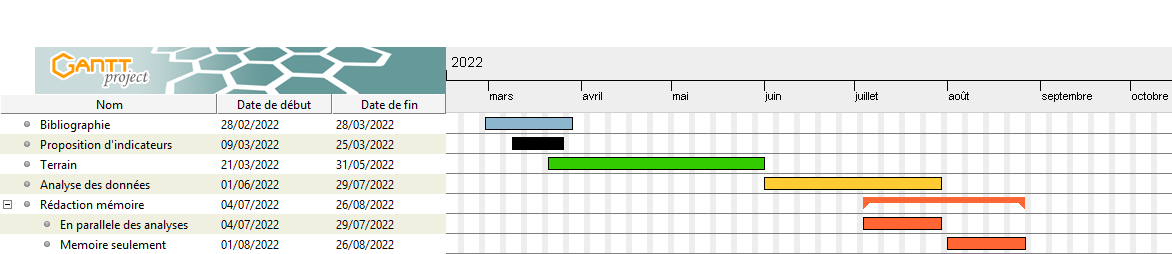
\includegraphics[width=1\linewidth]{images/chronogramme} 

}

\caption{Chronogramme du stage}\label{fig:planning}
\end{figure}

\normalsize

Le terrain se fera dans les forêts de Paracou et Régina Saint-Georges, pour lesquelles des données d'inventaires des arbres adultes sont disponible, ainsi que des données issues du LiDAR, à partir desquels une pré-identification des zones de trouées est faite.

\textbf{Protocole d'échantillonnage :}

Les trouées de plus de 10m2 sont préalablement repérées via le MNC issu des données LiDAR. Ces trouées sont donc géo référencées. Lors de la phase terrain, chacune de ces trouées sera visitée. Un inventaire est réalisé dans les cas où un semencier d'une des espèces cibles est présent à proximité de la trouées, et (ou ?) si des individus de notre liste d'espèce se trouve au stade de régénération dans la trouée en question.

\textbf{Effort d'échantillonnage:}

En moyenne, 12 placettes d'inventaire sont réalisées en une journée 2 terrain avec 2 opérateurs.

12 semaines soit 60 jours de terrain sont prévus, une marge de quelques jours étant nécessaire du fait des conditions météorologiques. Ainsi, 720 placettes pourront, au maximum, être réalisées dans le cadre de ce stage. En plus de cet inventaire, seront intégrées à l'analyse les données de 2 stages de 2 mois réalisés en 2021(Pierre-Justin, 2021) et 2022(Van der Meersh,2022) selon le même protocole .

\textbf{Protocole d'inventaire :}
Les espèces inventoriées sont les suivantes: Dicorynia Guianensis, Quaela rosa, Eperua falcata, Eperua Grandiflora, Ruitzeriana albiflora, Peltogyne spp, Manilkara bidentata, Manilkara uberi, Serotinia rubra, Goupia Glabra, Bagassa guianensis, Vouacapoua americana.

Au niveau des trouées d'intérêt repérées via les données lidar, 4 placettes de 5m de rayon seront réalisées par trouées :

\begin{itemize}
\item
  Une placette aura pour centre la souche de l'arbre exploité(ou tombé naturellement ? que fait-on dans ce cas?)
\item
  Une 2\textsuperscript{e} aura pour centre le houppier de l'arbre
\item
  Une 3\textsuperscript{e} est placée en lisière du chablis
\item
  Une 4\textsuperscript{e} est placée à distance du chablis ( comment on choisit la distance au chablis?)
\end{itemize}

Dans chaque placette sont inventoriés les individus des 11 espèces présentant une hauteur supérieure à 30 cm et un diamètre inférieur à 10 cm:

\begin{itemize}
\item
  La hauteur de chaque individu est mesurée à l'aide d'un télémètre(?)
\item
  Le diamètre des tiges de plus de 1,3m de haut est mesuré au pied à coulisse.
\end{itemize}

La hauteur des 3 plus hautes tiges ne faisant pas partie de la liste d'espèces à inventorier est également mesurée. Cette mesure permet d'avoir une idée de la compétition entre nos espèces d'intérêt et les autres.

This template is based on \emph{Bookdown} and the \emph{Memoir} LaTeX class to allow writing a book, a report, a PhD thesis, etc. in \emph{R Markdown}.

The main file is \emph{index.Rmd} which contains the description of the book in its header. All other \emph{.Rmd} files in the folder contain a chapter.
The \emph{references.bib} file contains the bibliography.

This file will have to be deleted, as well as \emph{81-getting\_started.Rmd} and \emph{82-syntax.Rmd}: they have to be replaced by the content of the book.

To get started, create a new R project from this folder.
Then open \emph{index.Rmd} and click on the \emph{Build Book} button in the \emph{Build} window of Rstudio.


% Bibliography
%%%%%%%%%%%%%%%%%%%%%%%%%%%%%%%%%%%%%%%%%%%%%%%%%%%%%%%%%%

\backmatter
\SmallMargins

\printbibliography
\onecolumn


% Tables (of tables, of figures)
%%%%%%%%%%%%%%%%%%%%%%%%%%%%%%%%%%%%%%%%%%%%%%%%%%%%%%%%%%


\cleardoublepage
\LargeMargins
\listoffigures


% After-body (LaTeX code inclusion)
%%%%%%%%%%%%%%%%%%%%%%%%%%%%%%%%%%%%%%%%%%%%%%%%%%%%%%%%%%




% Back cover
%%%%%%%%%%%%%%%%%%%%%%%%%%%%%%%%%%%%%%%%%%%%%%%%%%%%%%%%%%%

% Even page, small margins, no running head, no page number.
\evenpage
\SmallMargins
\thispagestyle{empty}

\begin{normalsize}

\begin{description}

\selectlanguage{english}
\item[Abstract]
English abstract, on the last page.

This is a bookdown template based on LaTeX memoir class.
\item[Keywords]
Keyword in English, As a list.
~\\

\end{description}

\end{normalsize}

\vspace*{\fill}
\centering
\includegraphics[width=.3\textwidth]{images/logo}

\end{document}
